\chapter{Rešerše}
\label{chap:reserse}

Kapitola shrnuje současný stav poznání v~oblasti detekce anomálií v~šifrovaném síťovém provozu. Nejprve jsou popsány šifrovací protokoly a~taxonomie útoků zneužívajících šifrované kanály, poté metody hlubokého učení, klasického strojového učení a~statistické přístupy k~detekci anomálií. Závěrečná sekce provádí tematickou analýzu identifikovaných zdrojů podle metodiky \textcite{Braun2006} a~propojuje poznatky rešerše s~návrhem experimentu v~kapitole~\ref{chap:metodika}.

\section{Přehled šifrovacích protokolů a možných útoků}
\label{sec:prehled-sifrovani}

\subsection{Šifrovací protokoly TLS a VPN}
\label{sec:sifrovaci-algoritmy}

Komunikace na internetu využívá vrstvený model, v~němž každá vrstva přidává vlastní hlavičky a~zapouzdřuje obsah vrstev vyšších. Obrázek~\ref{fig:network-layers} znázorňuje vztah mezi vybranými protokoly a~vrstvami síťového modelu; uvedené protokoly jsou relevantní pro detekci anomálií, protože na každé vrstvě jsou dostupná odlišná metadata.

\begin{figure}[htbp]
\centering
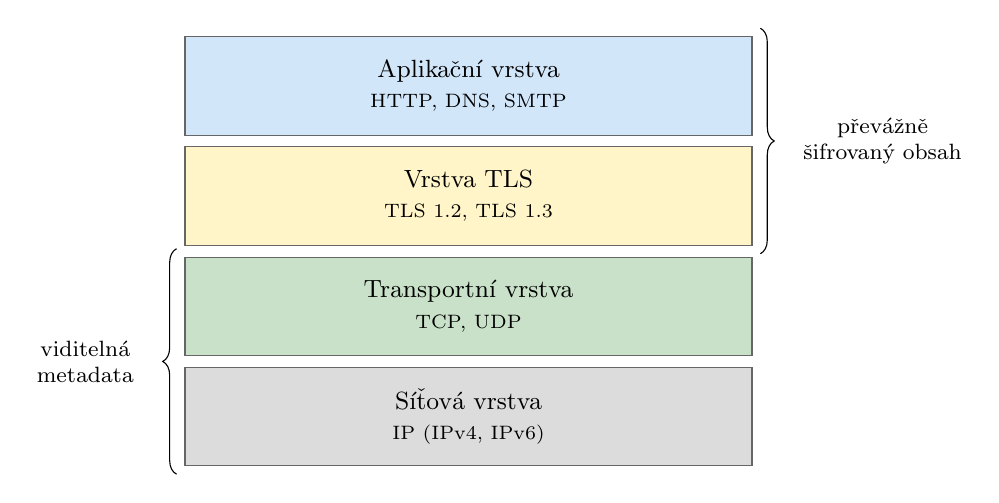
\begin{tikzpicture}[
  layer/.style={
    draw=black!60,
    minimum width=7.2cm,
    minimum height=1.25cm,
    font=\small,
    align=center,
    inner sep=4pt
  },
  bracelabel/.style={
    font=\footnotesize,
    align=center
  }
]

\definecolor{L4col}{RGB}{210,230,250}
\definecolor{L3col}{RGB}{200,225,200}
\definecolor{L2col}{RGB}{255,245,200}
\definecolor{L1col}{RGB}{220,220,220}

\node[layer, fill=L4col] (app) at (0,0)
  {Aplikační vrstva\\{\scriptsize HTTP, DNS, SMTP}};
\node[layer, fill=L2col] (tls) at (0,-1.4)
  {Vrstva TLS\\{\scriptsize TLS~1.2, TLS~1.3}};
\node[layer, fill=L3col] (trans) at (0,-2.8)
  {Transportní vrstva\\{\scriptsize TCP, UDP}};
\node[layer, fill=L1col] (net) at (0,-4.2)
  {Síťová vrstva\\{\scriptsize IP (IPv4, IPv6)}};

\path (net.south west) ++(-0.10,-0.10) coordinate (braceLbot);
\path (trans.north west) ++(-0.10,0.10) coordinate (braceLtop);
\draw[decorate, decoration={brace, amplitude=5pt}]
  (braceLbot) -- (braceLtop)
  node[midway, anchor=east, xshift=0-12pt, bracelabel]
  {viditelná\\metadata};

\path (tls.south east) ++(0.10,-0.10) coordinate (braceRbot);
\path (app.north east) ++(0.10,0.10) coordinate (braceRtop);
\draw[decorate, decoration={brace, amplitude=5pt, mirror}]
  (braceRbot) -- (braceRtop)
  node[midway, anchor=west, xshift=12pt, bracelabel]
  {převážně\\šifrovaný obsah};

\end{tikzpicture}
\caption[Vrstvový model síťové komunikace a umístění vybraných protokolů]{Vrstvový model síťové komunikace a schematické umístění vybraných protokolů. Vygenerováno pomocí Claude Opus 4.6 \parencite{Anthropic2025}.}
\label{fig:network-layers}
\end{figure}

TLS je v~současnosti dominantním standardem pro šifrování komunikace na internetu; zajišťuje důvěrnost a~integritu dat přenášených mezi klientem a~serverem prostřednictvím kombinace asymetrické a~symetrické kryptografie \parencite{Keshkeh2021}. Přechod od verze~1.2 k~verzi~1.3 přinesl zásadní změny s~přímými důsledky pro možnosti analýzy síťového provozu.

TLS~1.2, standardizovaný v~roce 2008, podporoval širokou nabídku šifrovacích sad, tedy kombinací algoritmů pro výměnu klíčů (RSA, DHE, ECDHE), symetrické šifrování (AES-CBC, AES-GCM, RC4, 3DES) a~hashování (SHA-1, SHA-256). Tato flexibilita vedla k~nasazení konfigurací se slabými parametry, například statickému RSA klíčovému transportu bez dopředné utajitelnosti \parencite{Keshkeh2021}.

TLS~1.3, standardizovaný v~roce 2018, povoluje pouze tři šifrovací sady, přičemž všechny tři jsou postaveny na AEAD: \path{TLS_AES_128_GCM_SHA256}, \path{TLS_AES_256_GCM_SHA384} a~\path{TLS_CHACHA20_POLY1305_SHA256}. Dopředná utajitelnost prostřednictvím efemérních klíčů (X25519 nebo P-256) je povinná, čímž se eliminuje možnost zpětného dešifrování zachyceného provozu. Odvozování klíčů využívá HKDF s~explicitně oddělenými fázemi (early secret, handshake secret, application traffic secret), což zpřehledňuje kryptografický návrh oproti staršímu modelu PRF v~TLS~1.2 \parencite{Keshkeh2021}.

\begin{table}[htbp]
\centering
\caption{Přehled vybraných kryptografických algoritmů v~kontextu TLS a~VPN}
\label{tab:krypto-algoritmy}
\small
\begin{tabular}{p{2.85cm}p{3.05cm}p{4.85cm}p{2.75cm}}
\toprule
Algoritmus & Typ & Role v~TLS/VPN & Délka klíče / doména \\
\midrule
AES-128-GCM & AEAD (bloková šifra) & Záznamová ochrana dat (TLS~1.3) & 128 bit \\
AES-256-GCM & AEAD (bloková šifra) & Záznamová ochrana dat (TLS~1.3, VPN) & 256 bit \\
ChaCha20-Poly1305 & AEAD (proudová šifra) & Alternativa k~AES-GCM (TLS~1.3, WireGuard) & 256 bit klíč \\
RSA & asymetrická & Statický transport klíče (TLS~1.2); v~TLS~1.3 pro výměnu klíčů nepřípustný & 2048+ bit \\
ECDHE (X25519, P-256) & asymetrická, DH & Dočasná výměna klíčů, dopředná utajitelnost & křivky NIST/Curve25519 \\
HKDF & KDF & Odvození klíčů z~sdíleného tajemství (TLS~1.3) & SHA-256 / SHA-384 \\
SHA-256 / SHA-384 & hash & Integrita handshake a~KDF & 256 / 384 bit výstup \\
\bottomrule
\end{tabular}
\end{table}
Z~hlediska analýzy provozu je podstatné, že TLS~1.3 šifruje výrazně větší část handshake než jeho předchůdce: serverový certifikát a~rozšíření jsou chráněny handshake klíči, čímž se snižuje objem metadat dostupných pasivnímu pozorovateli \parencite{Ji2024}. Z~vnějšku tak nelze přímo zjistit, jaké šifrovací parametry byly mezi klientem a~serverem dohodnuty. Handshake TLS~1.3 vyžaduje pouze 1-RTT oproti dvěma u~TLS~1.2 a~umožňuje režim 0-RTT pro obnovená spojení, což snižuje latenci, ale přináší riziko opakovaných útoků (replay attacks).

Vývoj kryptografických algoritmů přitom stále akceleruje -- moderní šifrovací primitiva jsou navrhována s~ohledem na odolnost vůči kvantovým útokům a~zároveň na efektivní hardwarovou implementaci \parencite{Goswami2020}. Tato evoluce má přímý dopad na analýzu provozu, protože každé zúžení viditelných metadat vyžaduje sofistikovanější detekční přístupy.

Kromě TLS na aplikační úrovni šifrují síťovou komunikaci i~protokoly VPN, které operují na síťové úrovni a~zapouzdřují celý IP provoz. Tabulka~\ref{tab:krypto-algoritmy} uvádí algoritmy používané oběma třídami protokolů. VPN přidává další úroveň zapouzdření, která ztěžuje extrakci příznaků -- pozorovatel vidí pouze vnější IP hlavičky tunelu, nikoliv původní adresy a~porty komunikujících stran. Klasifikace VPN provozu podle aplikací je proto aktivním výzkumným tématem. \textcite{Almuhammadi2025} ukazují, že kombinace metod strojového učení a hlubokého učení dokáže efektivně rozlišit VPN a~non-VPN provoz i~bez~inspekce obsahu paketů, přičemž upozorňují na~nutnost zachování soukromí uživatelů při~sběru trénovacích dat.

\subsection{Hrozby šifrovaného provozu}
\label{sec:taxonomie-utoku}

Šifrované kanály slouží nejen k~ochraně legitimní komunikace, ale zneužívají je i~útočníci. \textcite{Ferdous2023} identifikují několik hlavních kategorií takových hrozeb. Společným rysem je využívání C2 serverů, s~nimiž malware komunikuje přes šifrované spojení, čímž se C2 provoz stává obtížně odlišitelným od legitimního HTTPS provozu.

\begin{itemize}
\item Ransomware patří mezi nejzávažnější hrozby; útočníci šifrují data obětí a~komunikaci s~C2 servery vedou přes TLS.
\item Cryptojacking, tedy nelegitimní těžba kryptoměn na napadených zařízeních, využívá šifrovanou komunikaci s~těžebními pooly a~v~posledních letech zaznamenal trojciferný nárůst v~některých odvětvích.
\item Bezsouborový malware (fileless malware) operuje výhradně v~paměti, využívá legitimní systémové nástroje (PowerShell, WMI) a~komunikaci s~C2 infrastrukturou vede přes šifrované kanály. Nezanechává tradiční artefakty na disku, a~je proto obzvláště obtížně detekovatelný.
\item Útoky na dodavatelský řetězec kompromitují důvěryhodné softwarové aktualizační mechanismy a~využívají šifrovaná spojení k~distribuci škodlivého kódu; provoz je legitimními certifikáty ověřen jako důvěryhodný \parencite{Ferdous2023}.
\item Domain fronting umožňuje maskovat skutečnou cílovou doménu C2 serveru využitím infrastruktury CDN: v~TLS SNI figuruje legitimní doména, zatímco skutečný HTTP požadavek směřuje na server útočníka.
\item DNS over HTTPS přesouvá DNS dotazy do šifrovaného kanálu, čímž ztěžuje detekci DNS tunelování a~exfiltrace dat \parencite{Papadogiannaki2022}.
\item V~oblasti IoT malware jako Mirai a~jeho varianty stále častěji využívají šifrované C2 kanály. IoT zařízení s~omezenými výpočetními zdroji představují specifickou výzvu, protože standardní bezpečnostní řešení na nich nelze provozovat \parencite{Ferdous2023}.
\end{itemize}

Společným jmenovatelem uvedených hrozeb je, že šifrování -- původně navržené k~ochraně uživatelů -- slouží útočníkům jako prostředek k~maskování škodlivé aktivity před bezpečnostními nástroji založenými na inspekci obsahu.

\subsection{Detekce hrozeb bez dešifrování: typologie a~výzvy}
\label{sec:pristupy-identifikace}

\textcite{OzkanOkay2021} rozlišují tři základní kategorie systémů detekce průniku:

\begin{itemize}
\item Signaturové IDS vyhledávají známé vzory útoků v~obsahu paketů.
\item Anomáliové IDS modelují normální chování síťového provozu a~detekují odchylky od tohoto modelu.
\item Hybridní systémy oba přístupy kombinují.
\end{itemize}

V~šifrovaném prostředí tato typologie naráží na~vrozené omezení signaturových přístupů: obsah paketů je pro pasivního pozorovatele nečitelný, takže klasická DPI ztrácí oporu. Pozornost se proto přesouvá k~anomáliovým a~hybridním přístupům, které pracují výhradně s~metadaty a~statistickými příznaky toků popsanými v~sekci~\ref{sec:sifrovana-komunikace}. Právě schopnost modelovat normální chování provozu z~metadat -- bez přístupu k~dešifrovanému obsahu -- staví detekci anomálií do role dominantní strategie pro šifrované sítě.

Anomáliové detektory lze dále dělit podle algoritmického základu, s~nímž modelují normální chování a~odchylky od něj. Práce se opírá o~tří-skupinové dělení, které prochází celým textem: metody hlubokého učení (sekce~\ref{sec:metody-dl}), klasického strojového učení (sekce~\ref{sec:klasicke-ml}) a~statistické či heuristické přístupy (sekce~\ref{sec:stat-metody}). Tyto tři skupiny se liší v~požadavcích na~anotovaná data, ve~výpočetních nárocích i~v~míře interpretovatelnosti; rozdíly mezi nimi tvoří hlavní osu zájmu této práce a~jsou empiricky zkoumány v~kontrolovaném experimentu (kapitola~\ref{chap:metodika}).

Nasazení anomáliových detektorů ve~skutečném provozu nicméně doprovázejí průřezové výzvy, které se projevují napříč všemi třemi skupinami a~motivují volbu vlastního experimentu na~shodných datech. Srovnatelnost studií komplikuje heterogenita veřejně dostupných datových sad -- každá studie často pracuje s~jinou sadou, jinou taxonomií útoků a~jiným příznakovým prostorem, takže přímé porovnání publikovaných metrik je zavádějící \parencite{Ji2024}. Interpretovatelnost modelů je v~bezpečnostním kontextu ceněná, avšak transparentnější výstupy samy o~sobě přinášejí riziko zneužití útočníky ke~konstrukci obcházejících vzorců, jak ve~svém přehledu upozorňují \textcite{Capuano2022}. Výkonnost modelů se navíc v~čase postupně zhoršuje v~důsledku změn statistických vlastností provozu (concept drift), což si vynucuje průběžnou aktualizaci a~ověřování \parencite{Qing2025}. Tyto výzvy slouží v~dalších sekcích kapitoly jako interpretační rámec; jednotlivé skupiny metod jsou popsány nejen z~hlediska algoritmu, ale i~s~ohledem na~to, jak se s~nimi vyrovnávají.

\section{Šifrovaná síťová komunikace, metadata a příznaky}
\label{sec:sifrovana-komunikace}

\subsection{Příznaky na úrovni jednotlivých paketů}
\label{sec:metadata}

I~při plně šifrovaném obsahu paketů zůstává řada informací přístupná pasivnímu pozorovateli. Tato metadata tvoří základ příznaků pro veškeré detekční metody diskutované v~dalších sekcích. Obrázek~\ref{fig:packet-structure} znázorňuje zapouzdření vrstev v~typickém HTTPS paketu a~vyznačuje, které části jsou čitelné bez dešifrování.

\begin{figure}[htbp]
\centering
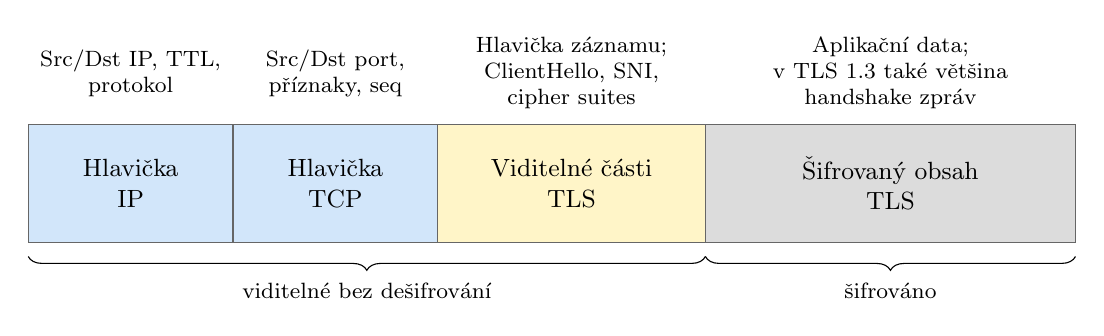
\begin{tikzpicture}[
  info/.style={font=\footnotesize, align=center}
]

\definecolor{visiblecol}{RGB}{210,230,250}
\definecolor{partialcol}{RGB}{255,245,200}
\definecolor{encryptedcol}{RGB}{220,220,220}

% Bloky paketu
\draw[fill=visiblecol, draw=black!60] (0,0) rectangle (2.6,1.5);
\node[align=center, font=\small] at (1.3,0.75) {Hlavička\\IP};

\draw[fill=visiblecol, draw=black!60] (2.6,0) rectangle (5.2,1.5);
\node[align=center, font=\small] at (3.9,0.75) {Hlavička\\TCP};

\draw[fill=partialcol, draw=black!60] (5.2,0) rectangle (8.6,1.5);
\node[align=center, font=\small] at (6.9,0.75) {Viditelné části\\TLS};

\draw[fill=encryptedcol, draw=black!60] (8.6,0) rectangle (13.3,1.5);
\node[align=center, font=\small] at (10.95,0.75) {Šifrovaný obsah\\TLS};

% Popisky nahoře
\node[info] at (1.3,2.15) {Src/Dst IP, TTL,\\protokol};
\node[info] at (3.9,2.15) {Src/Dst port,\\příznaky, seq};
\node[info] at (6.9,2.15) {Hlavička záznamu;\\ClientHello, SNI,\\cipher suites};
\node[info] at (10.95,2.15) {Aplikační data;\\v TLS~1.3 také většina\\handshake zpráv};

% Závorky dole
\draw [decorate, decoration={brace, amplitude=5pt, mirror}]
  (0,-0.18) -- (8.6,-0.18)
  node [midway, below=6pt, font=\footnotesize] {viditelné bez dešifrování};

\draw [decorate, decoration={brace, amplitude=5pt, mirror}]
  (8.6,-0.18) -- (13.3,-0.18)
  node [midway, below=6pt, font=\footnotesize] {šifrováno};

\end{tikzpicture}
\caption[HTTPS paket: viditelné hlavičky a šifrovaný obsah]{Zjednodušené schéma HTTPS/TLS komunikace. Bez dešifrování jsou viditelné hlavičky IP a TCP a část metadat TLS, zatímco aplikační data a v TLS~1.3 také většina handshake zpráv zůstávají šifrované. Vygenerováno pomocí Claude Opus 4.6 \parencite{Anthropic2025}.}
\label{fig:packet-structure}
\end{figure}

Na paketové úrovni jsou dostupné hlavičky IP (zdrojová a~cílová adresa, protokol, TTL, velikost paketu) a~transportní hlavičky TCP/UDP (zdrojový a~cílový port, příznaky TCP, sekvenční čísla, velikost okna). Tyto údaje šifrování neovlivňuje, protože směrovací a~transportní informace musí zůstat čitelné pro správné doručení paketu \parencite{Ji2024}.

Z~protokolu TLS jsou před ustanovením šifrovaného kanálu viditelné parametry handshake. U~TLS~1.2 zahrnují verzi protokolu, nabízené šifrovací sady, rozšíření (extensions), hodnotu SNI identifikující cílový server a~serverový certifikát. U~TLS~1.3 je množství viditelných parametrů omezeno -- certifikát a~většina rozšíření jsou šifrovány, ale SNI a~zpráva Client Hello s~nabídkou šifrovacích sad zůstávají čitelné \parencite{Keshkeh2021}. Právě tyto parametry slouží jako vstup pro techniky otiskování TLS.

Jednou z~technik pro identifikaci aplikací a~potenciálně škodlivých klientů v~šifrovaném provozu je otiskování parametrů TLS. Metoda JA3 \parencite{Althouse2017} generuje otisk z~parametrů zprávy Client Hello. Otisk zahrnuje verzi TLS, nabízené šifrovací sady, rozšíření, eliptické křivky a~formáty bodů na křivkách. Doplňková metoda JA3S analogicky otiskuje odpověď serveru. Kombinace JA3 a~JA3S umožňuje identifikovat konkrétní klientské implementace i~v~případě, kdy útočníci mění IP adresy a~doménová jména.

Dalším zdrojem příznaků je analýza certifikátů. Přestože TLS~1.3 certifikáty šifruje, v~praxi je stále možné využít informace z~OCSP odpovědí a~pozorovat vzorce v~obnovování certifikátů, jejich životnosti a~hierarchii certifikačních autorit. Malwarové C2 servery typicky používají vlastnoručně podepsané certifikáty nebo certifikáty od specifických nízkonákladových autorit, což představuje využitelný detekční příznak \parencite{Keshkeh2021}.

Na aplikační úrovni jsou u~nešifrovaných protokolů dostupné hlavičky HTTP. U~HTTPS jsou tyto informace šifrovány, ale z~handshake a~DNS dotazů lze odvodit cílovou doménu. Velikosti a~časování zpráv zůstávají pozorovatelné i~u~šifrovaného provozu \parencite{Barut2020}.

Mezi další dostupná metadata patří informace z~DNS a~metadata na úrovni spojení, jako je počet současně otevřených spojení ke stejnému serveru nebo frekvence navazování nových spojení \parencite{OzkanOkay2021}.

\subsection{Příznaky na úrovni síťových toků}
\label{sec:charakteristiky-toku}

Síťový tok (flow) je definován jako sekvence paketů sdílejících společný identifikátor -- typicky pětici (zdrojová IP, cílová IP, zdrojový port, cílový port, protokol) -- v~rámci časového okna. Agregace paketů do toků umožňuje výpočet statistických příznaků, které zachycují chování komunikace na vyšší úrovni abstrakce \parencite{Ji2024}.

Nástroj CICFlowMeter, vyvinutý na Canadian Institute for Cybersecurity, extrahuje ze souborů pcap více než 80~příznaků v~obou směrech toku \parencite{Sharafaldin2018}. Mezi typické kategorie příznaků patří:

\begin{itemize}
\item Velikosti paketů: celková, minimální, maximální, průměrná a~směrodatná odchylka velikosti paketů v~dopředném a~zpětném směru.
\item Mezipaketové intervaly (IAT): průměr, směrodatná odchylka, minimum a~maximum času mezi po~sobě jdoucími pakety. Tyto příznaky jsou obzvláště cenné pro šifrovaný provoz, protože časování paketů šifrování neovlivňuje.
\item Trvání a~rychlost toku: celková doba trvání toku, počet bajtů za sekundu a~počet paketů za sekundu.
\item Příznaky TCP: počet paketů s~nastavenými příznaky SYN, FIN, RST, PSH, ACK a~URG, které indikují fázi a~stav spojení.
\item Objemové příznaky: celkový počet paketů a~bajtů v~každém směru, poměr dopředných a~zpětných paketů.
\end{itemize}

Statistické vlastnosti toků jsou využitelné pro detekci anomálií, protože různé typy provozu vykazují charakteristické vzorce. \textcite{Barut2020} ve~svém srovnání ukazují, že C2 komunikace malwaru se v~šifrovaném prostředí typicky odlišuje od legitimního provozu krátkou dobou trvání toků s~pravidelným intervalem opakování a~asymetrickými objemy v~jednotlivých směrech, zatímco legitimní HTTPS provoz vykazuje vyšší variabilitu danou interakcí uživatele.

Formáty exportu toků jako NetFlow \parencite{CiscoNetFlow}, IPFIX \parencite{RFC7011} a~sFlow \parencite{sFlowDatagram} umožňují sběr těchto statistik v~reálném čase na síťových zařízeních. Pro výzkumné účely jsou toky typicky získány zpětně z~archivních souborů pcap pomocí nástrojů jako CICFlowMeter nebo nfstream \parencite{Ferriyan2021}.

\section{Metody hlubokého učení pro detekci anomálií}
\label{sec:metody-dl}

Metody hlubokého učení přinášejí schopnost automaticky extrahovat příznaky ze surových nebo předzpracovaných dat bez nutnosti manuálního inženýrství příznaků. V~kontextu detekce anomálií v~síťovém provozu se uplatňují zejména konvoluční neuronové sítě, autoencodery, rekurentní sítě a~transformery.

\subsection{Konvoluční neuronové sítě}
\label{sec:nn-dl}

CNN byly původně navrženy pro zpracování obrazu, ale jednorozměrné varianty (1D-CNN) se osvědčily i~pro klasifikaci síťového provozu. 1D-CNN aplikuje konvoluční filtry na sekvenci příznaků toku a~extrahuje lokální vzorce -- například charakteristické kombinace velikostí paketů nebo časových intervalů. Výhodou CNN je nízká latence při klasifikaci díky paralelizovatelnosti konvolučních operací \parencite{Bakhshi2021}. \textcite{Barut2020} ve svém srovnání potvrzují, že CNN modely dosahují vysoké přesnosti při klasifikaci TLS šifrovaného malwaru na základě příznaků na úrovni toku a~zároveň umožňují akceleraci pomocí knihoven jako OpenVINO \parencite{IntelOpenVINO} pro nasazení v~reálném čase.

\subsection{Autoencodery}
\label{sec:autoencodery}

Autoencodery jsou neuronové sítě trénované k~rekonstrukci vstupních dat prostřednictvím bottleneck vrstvy (kompresní mezivrstvy). Pro detekci anomálií se autoencoder na normálním provozu trénuje; anomální toky vedou k~vysoké rekonstrukční chybě, protože model nedokáže věrně rekonstruovat vzorce, které se nepodobají trénovacím datům. Autoencodery se řadí mezi metody bez učitele, což je výhodné v~situacích, kdy nejsou dostupná anotovaná data o~útocích \parencite{Ji2024}. Variační autoencodery \parencite{Kingma2014} rozšiřují tento přístup o~pravděpodobnostní modelování latentního prostoru.

\subsection{Rekurentní modely}
\label{sec:rekurentni}

Síťový provoz je ze své podstaty sekvenční -- pakety přicházejí v~časovém pořadí a~vzorce chování se projevují v~čase. Rekurentní neuronové sítě a~jejich varianty jsou proto přirozenou volbou pro modelování časových závislostí v~síťových tocích.

LSTM sítě \parencite{Hochreiter1997} řeší problém mizejícího gradientu klasických RNN (situaci, kdy se při~zpětném šíření chyby přes mnoho kroků gradient exponenciálně zmenšuje a~síť se přestává učit dlouhodobé závislosti) pomocí mechanismu brán, zde konkrétně se třemi (vstupní, brány zapomínání a~výstupní), který umožňuje selektivně uchovávat a~zapomínat informace v~dlouhých sekvencích. V~kontextu síťového provozu LSTM zpracovává sekvence toků nebo paketů a~zachycuje závislosti mezi vzdálenými událostmi \parencite{Bakhshi2021}.

GRU \parencite{Cho2014} je zjednodušená varianta LSTM se dvěma branami (aktualizační a~resetovací) místo tří. GRU dosahuje srovnatelné přesnosti jako LSTM při nižších výpočetních nárocích a~kratší době trénování, což je výhodné pro zpracování velkých objemů síťového provozu. \textcite{Bakhshi2021} ukazují, že hybridní kombinace CNN a~GRU dosahuje nejlepších výsledků: CNN extrahuje lokální příznaky s~nízkou latencí a~GRU modeluje časové závislosti, čímž vzniká model kombinující silné stránky obou architektur.

\subsection{Transformery}
\label{sec:transformery}

Transformery a~modely s~mechanismem pozornosti \parencite{Vaswani2017} představují novější alternativu k~rekurentním sítím. Na rozdíl od RNN zpracovávají celou sekvenci paralelně a~mechanismem vzájemné pozornosti mezi pozicemi váží vztahy mezi libovolnými místy v~sekvenci. Model ET-BERT \parencite{Lin2022} aplikuje architekturu BERT \parencite{Devlin2019} na šifrovaný provoz. BERT je model předtrénovaný na velkém objemu neanotovaných dat, který se učí obousměrné kontextuální reprezentace pomocí maskování vstupních tokenů; při aplikaci na síťový provoz se tyto reprezentace datagramů následně doladí pro konkrétní klasifikační úlohu. Na datové sadě CSTNET-TLS~1.3 dosáhl ET-BERT F1 skóre 97,4\,\%, což představovalo zlepšení o~10~procentních bodů oproti předchozím metodám. Transformery jsou výpočetně náročnější než CNN a~LSTM, ale jejich schopnost zobecnění z~předtrénovaných reprezentací je činí perspektivním směrem výzkumu.

\section{Klasické strojové učení pro detekci anomálií}
\label{sec:klasicke-ml}

Metody klasického strojového učení se od hlubokého učení liší absencí vícevrstvých neuronových reprezentací. Pracují s~ručně navrženými příznaky nebo jejich lineárními transformacemi. V~kontextu detekce anomálií v~síťovém provozu se uplatňují metody redukce dimenzí, shlukování a~specifické algoritmy detekce odlehlých hodnot.

\subsection{Metody redukce dimenzí}
\label{sec:pca}

Síťové toky jsou typicky popsány desítkami až stovkami příznaků, z~nichž mnohé jsou vzájemně korelované nebo pro detekci anomálií nepodstatné. PCA hledá lineární transformaci, která maximalizuje rozptyl dat v~menším počtu dimenzí. Pro detekci anomálií se PCA využívá dvěma způsoby:
\begin{itemize}
\item Anomální toky se projektují mimo podprostor definovaný hlavními komponentami normálního provozu, takže rekonstrukční chyba slouží jako skóre anomálie.
\item PCA slouží jako předzpracování pro další detekční metody tím, že snižuje šum a~redundanci v~datech.
\end{itemize}
\noindent \textcite{Chapagain2022} demonstrují, že kombinace PCA se shlukováním K-means zlepšuje přesnost detekce průniku. Na datové sadě NSL-KDD tato kombinace dosáhla vyšší přesnosti než samotný K-means na plném příznakovém prostoru.

\subsection{Shlukování}
\label{sec:shlukovani}

Shlukovací metody rozdělují síťové toky do skupin na základě podobnosti příznaků bez nutnosti anotovaných dat. Anomální toky se typicky nacházejí v~malých nebo izolovaných shlucích, případně jsou identifikovány jako odlehlé body.

K-means je nejrozšířenější shlukovací algoritmus. Iterativně přiřazuje body k~nejbližšímu centroidu a~přepočítává centroidy jako průměry přiřazených bodů. Počet shluků $k$ se volí předem, typicky pomocí Elbow metody nebo Silhouette koeficientu. Pro detekci anomálií se toky přiřazené k~malým shlukům nebo s~velkou vzdáleností od nejbližšího centroidu označují jako podezřelé \parencite{Chapagain2022}.

\subsection{Izolační les}
\label{sec:isolation-forest}

Izolační les \parencite{Liu2008} je algoritmus specificky navržený pro detekci anomálií. Vychází z~principu, že anomálie jsou vzácné a~odlišné od většiny dat, a~proto je lze izolovat menším počtem náhodných rozdělení prostoru. Algoritmus buduje soubor izolačních stromů, kde každý strom náhodně vybírá příznak a~náhodnou rozdělovací hodnotu. Anomální body, které se nacházejí v~řídkých oblastech prostoru, jsou izolovány blíže ke~kořeni stromu -- stačí tedy menší počet rozdělení k~jejich oddělení, což odpovídá kratší průměrné cestě (path length) ke~kořeni a~vyššímu skóre anomálie. Izolační les nevyžaduje trénovací data s~anotací anomálií, škáluje se lineárně s~počtem dat a~funguje dobře i~ve vysokodimenzionálních prostorech -- na rozdíl od K-means není citlivý na metriku vzdálenosti v~prostoru s~mnoha dimenzemi.

\section{Statistické a heuristické metody detekce anomálií}
\label{sec:stat-metody}

Statistické a~heuristické metody detekce anomálií se vyznačují absencí učení parametrů z~dat (nebo pouze minimální kalibrací prahů) a~vysokou interpretovatelností.

\subsection{Prahové a distribucionální metody}
\label{sec:stat-detekce}

Prahové metody definují pro zvolené příznaky horní a~dolní meze na základě historických dat. Překročení prahu spouští poplach. Metoda je jednoduchá, rychlá a~snadno interpretovatelná, ale vyžaduje manuální kalibraci prahů a~nereaguje na komplexní vzorce rozložené přes více příznaků současně \parencite{Dutta2022}.

Entropie síťového provozu měří míru náhodnosti v~distribuci příznaků. Prudká změna entropie signalizuje anomálii. Entropické metody jsou výpočetně nenáročné a~vhodné pro detekci volumetrických útoků a~skenování \parencite{OzkanOkay2021}.

Statistické testy -- z-skóre, Grubbsův test (který hledá největší odlehlou hodnotu ve~vzorku dat za~předpokladu normálního rozložení) nebo Mahalanobisova vzdálenost -- kvantifikují, nakolik se pozorování odchyluje od~očekávaného rozložení. Mahalanobisova vzdálenost zohledňuje korelace mezi příznaky, a~je proto vhodnější než euklidovská vzdálenost pro multivariační data síťových toků. Výhodou statistických metod je transparentnost a~nízká výpočetní náročnost; nevýhodou je předpoklad o~konkrétním rozložení dat, který v~reálném provozu nemusí platit \parencite{Dutta2022}.

Baseline model představuje nejjednodušší přístup: definuje se profil normálního provozu a~každý nový tok se porovnává s~tímto profilem. Odchylky nad stanovenou mez jsou označeny jako anomálie. I~přes svou jednoduchost slouží v~literatuře jako referenční výchozí bod pro srovnání se složitějšími metodami \parencite{OzkanOkay2021}.

\subsection{Pravidlové systémy}
\label{sec:pravidlove}

Tradiční pravidlové systémy, jako Snort a~Suricata, definují signatury ve formě pravidel nad hlavičkami a~obsahem paketů. V~šifrovaném provozu jsou tyto systémy omezeny na pravidla nad metadaty. \textcite{Papadogiannaki2022} navrhují přístup založený na sekvencích paketů a~metadatech, který umožňuje detekci průniku i~v~šifrovaných sítích. Tento přístup je deterministický a~vysvětlitelný, ale vyžaduje ruční tvorbu pravidel a~nedokáže detekovat neznámé útoky.

\subsection{Kombinace detektorů}
\label{sec:kombinace}

Jednotlivé detekční metody mají odlišné silné stránky a~limity. V~praxi se proto tyto metody kombinují do tzv. ensemble detektorů, které agregují výstupy více nezávislých modelů. Nejjednodušší formou je hlasování většinou: tok je označen jako anomální, pokud ho většina zahrnutých detektorů klasifikuje jako anomální. Tento přístup nevyžaduje další trénování a~může zvýšit robustnost detekce snížením závislosti na specifických předpokladech jednoho algoritmu. Ensemble metody jsou v~literatuře obecně považovány za efektivní strategii pro snížení míry falešných poplachů při zachování vysoké úplnosti \parencite{OzkanOkay2021}.

\section{Režimy učení a~průřezové výzvy}
\label{sec:rezimy-uceni}

Režim učení (supervision) představuje ortogonální dimenzi vůči třem skupinám metod zavedeným v~předchozích sekcích: detektor lze trénovat s~učitelem, bez učitele nebo částečně řízeným způsobem nezávisle na tom, zda využívá hlubokou neuronovou síť, klasický algoritmus strojového učení, nebo statistický test. Následující přehled shrnuje vlastnosti jednotlivých režimů a~společné výzvy, které se projevují napříč všemi třemi skupinami.

Učení s~učitelem vyžaduje anotovaná data -- dvojice (příznaky toku, třída). Na šifrovaných datových sadách dosahují nejvyšších hodnot F1~skóre jednak neuronové sítě z~hlubokého učení (CNN, LSTM, transformery), jednak vybrané algoritmy klasického strojového učení s~učitelem, které v~experimentu \textcite{Barut2020} překračují 99\,\% přesnosti. Společnou nevýhodou je závislost na kvalitě a~aktuálnosti anotovaných dat.

Učení bez učitele nevyžaduje anotovaná data a~detekuje anomálie jako odchylky od naučeného modelu normálního provozu. Z~hlubokého učení sem patří autoencodery, z~klasického strojového učení například K-means a~izolační les, mezi statistické a~heuristické zástupce patří prahové a~distribucionální testy. Tyto metody dokážou detekovat i~dosud neznámé útoky, ale obvykle vykazují vyšší míru falešných poplachů \parencite{Ji2024}.

Částečně řízené učení kombinuje malé množství anotovaných dat s~velkým objemem neanotovaných dat. Předtrénované modely typu ET-BERT \parencite{Lin2022} jsou příkladem z~rodiny hlubokého učení, obdobně lze v~klasickém strojovém učení využít samo-označování pomocí shlukovacích metod. Tento přístup je prakticky relevantní, protože získávání anotovaných dat o~útocích je nákladné a~časově náročné.

Napříč všemi třemi skupinami se projevují tři průřezové výzvy. První je nevyváženost datových sad -- legitimní provoz výrazně převažuje nad škodlivým, takže trénovací postupy musí využívat techniky jako SMOTE (syntetické převzorkování menšinové třídy), podvzorkování převažující třídy nebo váženou ztrátovou funkci \parencite{OzkanOkay2021}. Tento problém zasahuje všechny metody s~učitelem a~zvlášť citelně se projevuje u~parametricky bohatých neuronových sítí. Druhou výzvou je concept drift, kdy se charakter síťového provozu mění v~důsledku nasazení nových aplikací, změn chování uživatelů nebo aktualizací protokolů; modely trénované na starších datech v~důsledku toho postupně ztrácejí přesnost \parencite{Qing2025}. Třetí výzvou jsou adversariální útoky na samotný detektor, především tzv.~evasion útoky: útočník záměrně mírně pozmění metadata škodlivého toku tak, aby ho detektor klasifikoval jako normální provoz. Na rozdíl od útoků popsaných v~sekci~\ref{sec:taxonomie-utoku}, které jsou vedeny přes šifrovaný kanál proti uživateli nebo organizaci, evasion útoky cílí na klasifikační model. Gradientní varianta zneužívá diferencovatelnosti neuronových sítí -- útočník spočítá směr minimální úpravy vstupu, která překlopí rozhodnutí modelu, a~je proto účinná především proti hlubokému učení. Modely, které diferencovatelné nejsou (statistické testy, stromy, izolační les), gradientním útokům odolávají, ale zůstávají zranitelné dotazovacími (black-box) a~mimikovacími útoky, při nichž jsou statistiky škodlivého toku upraveny tak, aby napodobovaly legitimní provoz \parencite{He2023}. Všechny tři výzvy motivují pravidelné přetrénování, použití více nezávislých detektorů a~slouží jako interpretační rámec pro diskusi výsledků v~kapitole~\ref{chap:vysledky}.

\section{Tematická analýza výsledků rešerše}
\label{sec:tematicka-analyza}

Rešerše v~předchozích sekcích identifikovala řadu metod a~přístupů k~detekci anomálií v~šifrovaném provozu, které se liší algoritmickým základem, požadavky na data i~hlášenými výsledky. Pro systematické zpracování těchto poznatků a~jejich propojení s~návrhem experimentu v~kapitole~\ref{chap:metodika} je zapotřebí analytický rámec, který umožní kategorizovat existující přístupy a~identifikovat opakující se vzorce. Tematická analýza podle Brauna a~Clarka \parencite{Braun2006} byla zvolena, protože poskytuje flexibilní a~transparentní postup pro kvalitativní zpracování heterogenního souboru vědeckých prací. Na rozdíl od čistě kvantitativních meta-analýz, které vyžadují srovnatelné numerické výsledky, umožňuje tematická analýza pracovat s~různorodými studiemi lišícími se metodologií, datovou sadou i~měřenými metrikami. Výstupem je kódovací rámec mapující analyzované práce na témata, čímž vzniká strukturovaný podklad pro výběr metod a~návrh experimentu v~praktické části.

\subsection{Metoda a~postup}
\label{sec:ta-metoda}

Braun a~Clarke \parencite{Braun2006} definují šest fází tematické analýzy; v~následujícím textu je popsáno, jak byly tyto fáze aplikovány na rešerši provedenou v~předchozích sekcích.

\begin{enumerate}
\item Seznámení s~daty:

Všechny články zahrnuté do rešerše (viz sekce~\ref{sec:prehled-sifrovani} až~\ref{sec:stat-metody}) byly přečteny s~cílem identifikovat pasáže relevantní pro detekci anomálií v~šifrovaném provozu. Při čtení byly poznamenávány klíčové koncepty: jakou míru supervize metoda vyžaduje, na jaké úrovni abstrakce dat operuje, jak důkladně jsou výsledky validovány a~zda autoři diskutují provozní aspekty nasazení.

\item Konstrukce předběžných kódů:

Z~poznámek vznikly kódy jako učení s~učitelem, učení bez učitele, částečně řízené učení, metadata handshake, statistiky toků, surové bajty, jedna datová sada, cross-dataset validace, concept drift, výpočetní nároky, latence, interpretovatelnost, soukromí, adversariální robustnost a~další. Kódy byly přiřazeny ke konkrétním pasážím prací.

\item Hledání témat:

Kódy byly seskupeny podle konceptuální blízkosti. Kódy učení s~učitelem, bez učitele a~částečně řízené se seskupily do tématu popisujícího míru supervize. Kódy metadata handshake, statistiky toků a~surové bajty vytvořily téma úroveň vstupních příznaků. Kódy jedna datová sada, cross-dataset a~concept drift zformovaly téma důkladnost validace. Kódy výpočetní nároky, interpretovatelnost a~soukromí se seskupily do tématu provozní nasaditelnost.

\item Revize témat:

Kandidátská témata byla přezkoumána z~hlediska vnitřní koherence a~vzájemného rozlišení. Původní téma \uv{typ detekčního přístupu} (CNN vs. PCA vs. pravidlové IDS) bylo vyřazeno jako příliš obecné, protože všechny rešeršované zdroje byly vybrány právě proto, že se věnují detekčním přístupům -- téma by tak nerozlišovalo mezi zdroji. Místo toho bylo nahrazeno granulárním tématem T1 (míra supervize, viz sekce~\ref{sec:ta-temata}), které zachycuje klíčový praktický rozdíl mezi přístupy.

\item Definice a~pojmenování témat:

Finální čtyři témata jsou pojmenována a~definována v~následující podsekci.

\item Zpracování výstupu:

Výstupem je text této sekce včetně mapovací tabulky~\ref{tab:tematicka-analyza}, která vizualizuje pokrytí témat v~jednotlivých analyzovaných zdrojích.
\end{enumerate}

\subsection{Identifikovaná témata}
\label{sec:ta-temata}

Na základě rešerše byla vymezena čtyři hlavní témata:

\begin{description}
\item[T1 -- Míra supervize a~požadavky na anotovaná data.] Téma rozlišuje, zda metoda vyžaduje plně anotovaná trénovací data (učení s~učitelem), pouze data normálního provozu bez anotací (učení bez učitele), nebo malé množství anotovaných vzorků doplněné velkým objemem neanotovaných dat (částečně řízené učení). Míra supervize je klíčovým praktickým diferenciátorem, protože získávání anotovaných dat o~útocích je nákladné a~anotace rychle zastarávají s~vývojem nových hrozeb.

\item[T2 -- Typ a~úroveň abstrakce vstupních příznaků.] Téma rozlišuje, na jaké úrovni abstrakce metoda operuje: metadata TLS handshake, agregované statistiky toků, časové sekvence toků, nebo surové bajty. Úroveň příznaků určuje, jakou infrastrukturu pro sběr dat metoda vyžaduje, a~ovlivňuje přenositelnost výsledků mezi různými síťovými prostředími.

\item[T3 -- Metodologická důkladnost validace.] Téma zachycuje, jak důkladně jsou hlášené výsledky validovány: počet použitých datových sad, testování přenositelnosti mezi síťovými prostředími, zohlednění concept drift a~reprodukovatelnost experimentů. Rozdíly v~důkladnosti validace jsou podstatné pro správnou interpretaci rešeršních tvrzení.

\item[T4 -- Provozní nasaditelnost.] Téma zahrnuje aspekty přesahující čistou přesnost detekce: výpočetní nároky a~latenci při klasifikaci, interpretovatelnost modelů pro SOC operátory, ochranu soukromí uživatelů při analýze provozu a~odolnost vůči adversariálním vstupům. Tyto faktory ovlivňují, zda je nasazení metody v~reálném prostředí proveditelné.
\end{description}

\subsection{Syntéza a~závěry z~tematické analýzy}
\label{sec:ta-synteza}

Tabulka~\ref{tab:tematicka-analyza} mapuje klíčové práce citované v~předchozích sekcích na identifikovaná témata (T1--T4) definovaná v~předchozí podsekci. Symbol $\checkmark$ označuje, že dané téma v~práci výrazně vystupuje. Zdroje jsou řazeny chronologicky.

\begin{table}[htbp]
\centering
\caption{Mapování analyzovaných zdrojů na témata tematické analýzy}
\label{tab:tematicka-analyza}
\small
\setlength{\tabcolsep}{5pt}
\begin{tabular}{l@{\hspace{8pt}}c@{\hspace{8pt}}c@{\hspace{8pt}}c@{\hspace{8pt}}c}
\toprule
 & \shortstack{Míra\\supervize\\(T1)} & \shortstack{Vstupní\\příznaky\\(T2)} & \shortstack{Důkladnost\\validace\\(T3)} & \shortstack{Provozní\\nasaditelnost\\(T4)} \\
\midrule
\textcite{Liu2008}                       & \checkmark &            &            &            \\
\textcite{Sharafaldin2018}                &            & \checkmark &            &            \\
\textcite{Goswami2020}                   &            & \checkmark &            &            \\
\textcite{Barut2020}                     & \checkmark & \checkmark & \checkmark &            \\
\textcite{Bakhshi2021}                   & \checkmark & \checkmark & \checkmark & \checkmark \\
\textcite{Keshkeh2021}                   & \checkmark & \checkmark &            &            \\
\textcite{Ferriyan2021}                  &            & \checkmark & \checkmark &            \\
\textcite{OzkanOkay2021}                 & \checkmark & \checkmark & \checkmark & \checkmark \\
\textcite{Capuano2022}                   &            &            &            & \checkmark \\
\textcite{Priyadarshini2022}             &            &            &            & \checkmark \\
\textcite{Chapagain2022}                 & \checkmark & \checkmark & \checkmark &            \\
\textcite{Dutta2022}                     & \checkmark & \checkmark &            &            \\
\textcite{Lin2022}                       & \checkmark & \checkmark & \checkmark &            \\
\textcite{Papadogiannaki2022}             &            & \checkmark &            &            \\
\textcite{Ferdous2023}                   &            &            &            &            \\
\textcite{Ji2024}                        & \checkmark & \checkmark & \checkmark & \checkmark \\
\textcite{Almuhammadi2025}               & \checkmark & \checkmark & \checkmark & \checkmark \\
\textcite{Qing2025}                      & \checkmark & \checkmark & \checkmark &            \\
\bottomrule
\end{tabular}
\end{table}

Z~tabulky~\ref{tab:tematicka-analyza} a obsahů uvedených zdrojů vyplývá několik pozorování relevantních pro návrh experimentu v~kapitole~\ref{chap:metodika}.

Z~hlediska míry supervize (T1) převažují v~literatuře metody s~učitelem; přístupy bez učitele a~částečně řízené zastupují méně prací, přestože jsou prakticky relevantní v~situacích, kdy anotovaná data nejsou dostupná. Téma T2 (vstupní příznaky) pokrývá většina zdrojů -- příznaky na úrovni toku a~veřejné datové sady tvoří převažující vzorec výzkumu, zatímco přístupy pracující se surovými bajty zastupuje pouze jedna práce. To naznačuje, že agregované statistiky toků představují v~současnosti běžný způsob práce v oboru.

Důkladnost validace (T3) se mezi pracemi výrazně liší: od pouhého uvedení přesnosti na jedné datové sadě až po systematické srovnání napříč síťovými podmínkami s~diskusí concept drift. Tato nekonzistence ztěžuje přímé srovnání studií a~motivuje provedení vlastního kontrolovaného experimentu na shodné datové sadě, jak je navrženo v~kapitole~\ref{chap:metodika}.

Provozní nasaditelnost (T4) se výrazně objevuje pouze u~pěti prací, což naznačuje, že otázky výpočetních nároků, interpretovatelnosti a~soukromí jsou v~literatuře dosud nedostatečně reflektovány vzhledem k~jejich praktickému významu.

Propojení témat s~dílčími cíli práce je následující: systematické srovnání tří skupin metod (dílčí cíle~4 a~5) přímo odpovídá průsečíku témat T1 a~T3 -- experiment porovnává metody s~různou mírou supervize za kontrolovaných validačních podmínek. Návrh experimentálního prostředí a~implementace prototypu (dílčí cíle~2 a~3) se váže k~tématu T2 a~k~poznatku, že úroveň příznaků zásadně ovlivňuje srovnatelnost výsledků. Omezení a~provozní výzvy diskutované v~rešerši odpovídají tématu T4. Tematická analýza tak poskytuje strukturovaný základ pro návrh experimentu v~následujících kapitolách.

\section{Přehled metod detekce anomálií v šifrovaném provozu}
\label{sec:prehled-srovnani}

Předchozí podkapitoly podrobně popsaly jednotlivé třídy metod od statistických přístupů přes klasické strojové učení až po hluboké učení. Tato sekce shrnuje teoretické srovnání těchto přístupů na základě literatury, které slouží jako podklad pro empirické srovnání v~kontrolovaném experimentu v~kapitole~\ref{chap:metodika}. Níže jsou metody porovnány z~hlediska vlastností relevantních pro praktické nasazení.

Z~hlediska přesnosti detekce dosahují v~literatuře nejvyšších hodnot F1~skóre modely hlubokého učení s~učitelem (CNN, LSTM, transformery) a~dále vybrané algoritmy klasického strojového učení s~učitelem, které rovněž překračují 95\,\% na standardních datových sadách \parencite{Barut2020}. Modely bez učitele -- autoencodery z~hlubokého učení a~metody klasického strojového učení jako PCA, K-means či izolační les -- dosahují obvykle nižší přesnosti, ale nevyžadují anotovaná data a~dokážou detekovat neznámé útoky.

Výpočetní náročnost se výrazně liší. Statistické metody (prahování, entropie) a~pravidlové systémy mají zanedbatelnou režii a~jsou vhodné pro nasazení v reálném čase na síťových zařízeních. PCA a~K-means vyžadují minimální výpočetní zdroje po úvodní fázi trénování. Izolační les škáluje lineárně s~objemem dat. CNN má nízkou latenci při klasifikaci. LSTM a~GRU jsou sekvenční a~tedy pomalejší. Transformery jsou nejnáročnější na výpočetní zdroje, zejména ve fázi trénování \parencite{Bakhshi2021}.

Z~hlediska potřeby anotovaných dat lze metody seřadit: statistické a~pravidlové metody nepotřebují žádná trénovací data. Metody klasického strojového učení bez učitele (izolační les, K-means, PCA) a~autoencodery vyžadují pouze data normálního provozu. Částečně řízené přístupy (ET-BERT) potřebují malé množství anotovaných dat. Modely hlubokého učení s~učitelem (CNN, LSTM) vyžadují plně anotované datové sady.

Interpretovatelnost je vysoká u~statistických a~pravidlových metod, střední u~izolačního lesa (kde lze identifikovat klíčové příznaky) a~nízká u~hlubokých neuronových sítí. Nízká interpretovatelnost modelů hlubokého učení je problematická pro SOC~operátory, kteří potřebují porozumět důvodu poplachu. Metody XAI mohou interpretovatelnost zvýšit, ale přinášejí riziko zneužití útočníky, jak upozorňují \textcite{Capuano2022}.

Robustnost vůči postupné změně statistických vlastností provozu je slabinou modelů trénovaných na statických datových sadách. \textcite{Qing2025} ukazují, že standardní modely ztrácejí přesnost při změně síťových podmínek, a~navrhují jako řešení přístupy meta-učení, tedy modely schopné se rychle přizpůsobit novému rozložení dat z~malého počtu nových příkladů. Statistické metody s~adaptivními prahy se přizpůsobují přirozeně, pokud je baseline model pravidelně aktualizován.

Odolnost vůči evasion útokům (popsaným jako třetí průřezová výzva v~sekci~\ref{sec:rezimy-uceni}) je u~jednotlivých skupin metod odlišná. Modely hlubokého učení jsou častým cílem gradientní varianty, protože útočník může využít diferencovatelnosti sítě \parencite{He2023}. Statistické a~heuristické metody gradientním útokům odolávají, ale zůstávají zranitelné dotazovacími a~mimikovacími variantami. Kombinace více nezávislých detektorů celkovou odolnost zvyšuje, protože útočníkovi ztěžuje nalezení úpravy účinné proti všem modelům najednou \parencite{He2023}.

Literatura opakovaně zdůrazňuje, že v~bezpečnostním kontextu má úplnost detekce často větší váhu než přesnost, neboť nezachycený incident může mít závažnější důsledky než falešný poplach \parencite{OzkanOkay2021}. Přehled literatury současně ukazuje, že žádná jednotlivá metoda nepřevažuje ve všech hodnotících dimenzích: při dostatku anotovaných dat hluboké modely často dosahují vyšších hlášených skóre přesnosti, zatímco statistické metody nabízejí transparentnost a~nízkou výpočetní náročnost. Uvedené srovnání vychází z~tvrzení publikovaných v~analyzované literatuře a~je proto nutně zatíženo rozdíly v~datových sadách, metrikách a~experimentálních podmínkách jednotlivých studií. Empirické ověření těchto teoretických poznatků na shodné datové sadě za kontrolovaných podmínek je předmětem experimentu navrženého v~kapitole~\ref{chap:metodika}.
